% ARPEGOS:  Automatized Roleplaying-game Profile Extensible Generator Ontology based System %
% Author : Alejandro Muñoz Del Álamo %
% Copyright 2019 %

% Section 4.4: Modelo de Interfaz de Usuario %
\section{Modelo de Interfaz de Usuario}
En esta sección se trata la interacción entre el sistema y el usuario a través de las diferentes vistas 
de las que dispone el sistema.

\subsection{Pantalla de inicio}
La pantalla de inicio de la aplicación se muestra cuando la aplicación se inicia. En ella se 
muestran los diferentes juegos actualmente disponibles para la aplicación.
Dispone de dos iconos interactivos en la esquina superior derecha de la pantalla, para añadir o eliminar 
juegos en la aplicación, y un menú contextual, que se puede activar pulsando sobre el icono dispuesto 
en la esquina superior izquierda de la pantalla. Esta vista se puede apreciar en la figura \ref*{PantallaInicio}.
\newpage

\begin{figure}[H]
    \centering
    \begin{minipage}{0.38\textwidth}
        \centering
        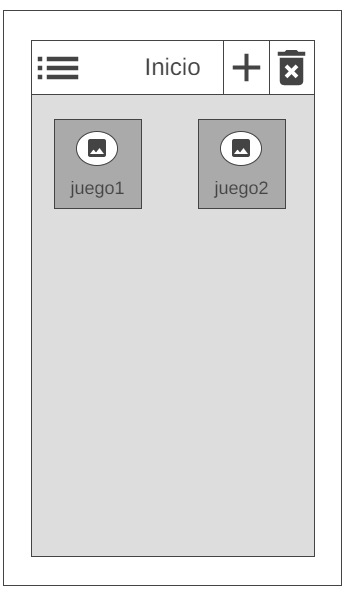
\includegraphics[scale=0.5]{Figures/Mockups/Mock_Inicio.png}
        \caption{Pantalla de inicio}
        \label{PantallaInicio}    
    \end{minipage} \hspace{2cm}
    \begin{minipage}{0.38\textwidth}   
        \centering
        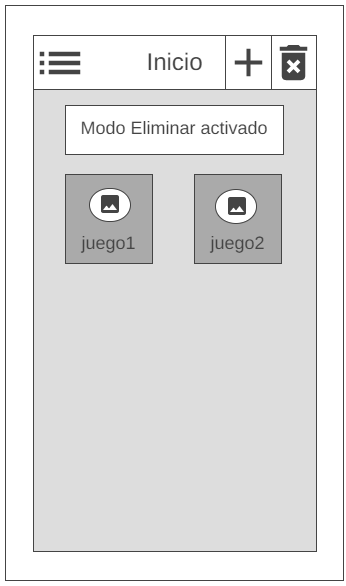
\includegraphics[scale=0.5]{Figures/Mockups/Mock_Eliminar.png}
        \caption{Modo de eliminación}
        \label{ModoEliminacion}    
    \end{minipage}
\end{figure}


En el caso de que el usuario desee eliminar uno o varios de los juegos existentes, al pulsar sobre el 
icono de la papelera, surgirá un aviso indicando que está activado el modo de eliminación, de manera que 
al seleccionar un elemento, en vez de acceder a su contenido, lo estará seleccionando para eliminarlo, tal 
y como se muestra en la figura \ref*{ModoEliminacion}. Al seleccionar un juego para eliminarlo, 
la aplicación realizará una pregunta de seguridad, ya que una vez eliminado el juego, no será posible 
recuperarlo.


\subsection{Pantalla de adición de juego}
A esta vista se puede acceder al pulsar sobre el icono de adición en la esquina superior derecha 
de las pantallas de inicio, y de selección de versión. Esta vista dispone de un icono de flecha en la esquina superior 
izquierda de la pantalla en caso de que se desee volver a la vista previa. En el centro de la pantalla se pueden apreciar 
una caja de texto y tres botones, llamados \textit{Comprobar juego}, \textit{Seleccionar fichero} y \textit{Añadir fichero} 
(figura \ref*{AnadirJuego}).
\newpage
\begin{figure}[H]
    \centering
    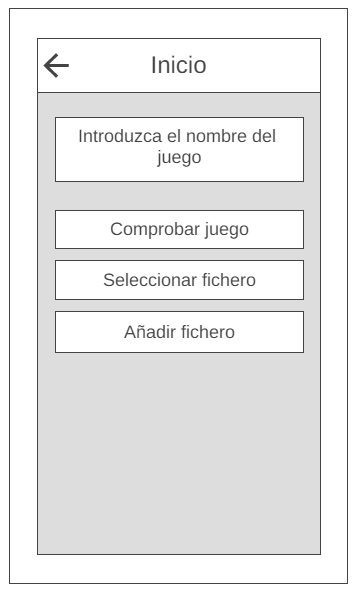
\includegraphics[scale=0.4]{Figures/Mockups/Mock_AnadirJuego.png}
    \caption{Adición de juego}
    \label{AnadirJuego}    
\end{figure}

%En primer lugar, aparece una caja de texto, en la que podemos introducir el nombre del juego que queremos añadir.
%A continuación se encuentra el botón \textit{Comprobar juego}, el cual creará la estructura del juego indicado en caso 
%de no existir (figura \ref*{ComprobarJuego}). En caso contrario, indicará que dicho juego ya existe. 
%
%\begin{figure}[H]
%    \centering
%    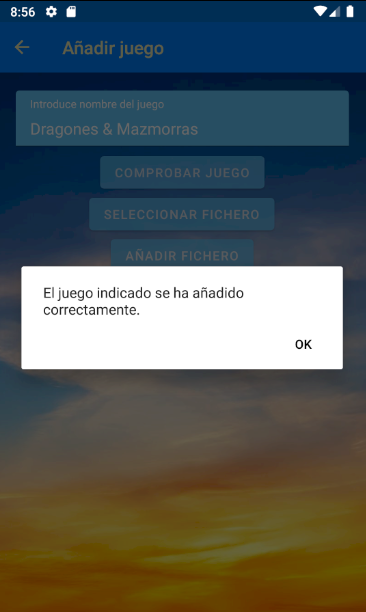
\includegraphics[scale=0.4]{Figures/Capturas/ComprobarJuego.png}
%    \caption{Comprobar juego}
%    \label{ComprobarJuego}    
%\end{figure}
%
%Seguidamente está dispuesto el botón \textit{Seleccionar fichero}, que permite al usuario indicar el fichero en el que se 
%encuentra la información del juego, haciendo uso del sistema de ficheros del dispositivo (figura \ref*{SeleccionarFichero1}). 
%Una vez seleccionado, el sistema mostrará por pantalla un aviso indicando cuál es el fichero seleccionado.
%
%\begin{figure}[H]
%    \centering
%    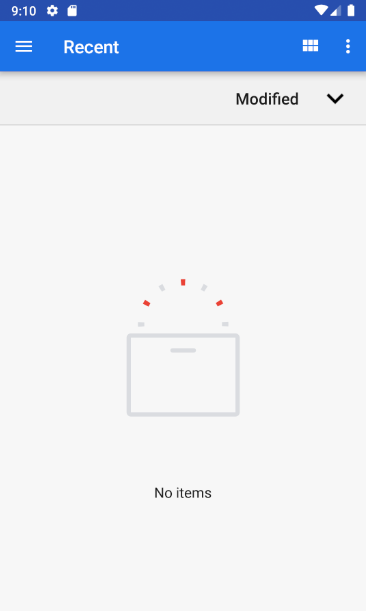
\includegraphics[scale=0.4]{Figures/Capturas/SistemaFicheros.png}
%    \caption{Búsqueda de fichero}
%    \label{SeleccionarFichero1}    
%\end{figure}
%
%En último lugar está el botón \textit{Añadir fichero}, que introduce el fichero previamente 
%seleccionado en la carpeta del juego indicado en la caja de texto, y muestra un aviso por pantalla indicando si 
%el fichero se ha añadido exitosamente.

\subsection{Menú contextual}
El menú contextual consiste en una vista oculta en la aplicación que se despliega al pulsar un icono de 
tres barras horizontales, ubicado en la esquina superior izquierda de la pantalla.\medskip

Al abrir el menú contextual se muestran tres opciones: \textit{Inicio}, \textit{Seleccionar personaje} y 
\textit{Seleccionar tema}. La primera opción hace que la aplicación retroceda a la pantalla de inicio.
La segunda lleva al usuario a la vista de selección de personaje, siempre y cuando el juego esté seleccionado. 
En caso contrario, el sistema lanzará una alerta avisando que no es posible seleccionar personajes mientras no 
se haya escogido un juego previamente (figura \ref*{MenuContextual}). Por último, la tercera opción abre la vista de 
selección de tema.

\begin{figure}[H]
    \centering
    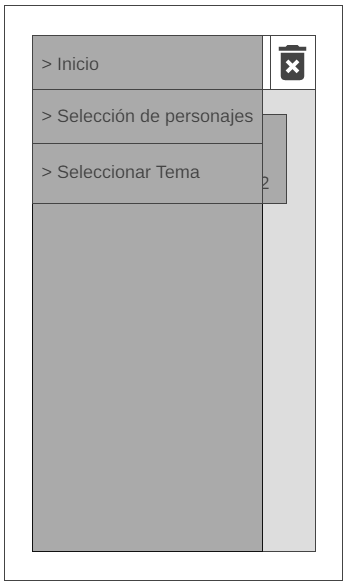
\includegraphics[scale=0.4]{Figures/Mockups/Mock_Menu.png}
    \caption{Menú contextual}
    \label{MenuContextual}    
\end{figure}

\subsection{Pantalla de selección de tema}
Esta vista sólo es accesible desde la opción \textit{Seleccionar tema} del menú contextual.
En ella se mostrarán las diversas opciones de temas de fondo, y un color, referente al color base del tema cuyo nombre acompaña.

\begin{figure}[H]
    \centering
    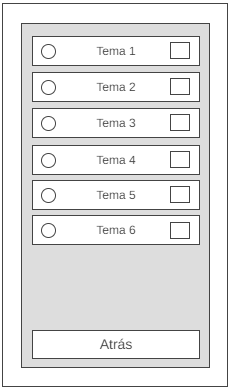
\includegraphics[scale=0.5]{Figures/Mockups/Mock_SeleccionTema.png}
    \caption{Selección de tema}
    \label{SeleccionTema}    
\end{figure}
\newpage
\subsection{Pantalla de selección de versión}
La pantalla de selección de versión se muestra al seleccionar un juego en la pantalla de inicio.
Tiene la misma estructura visual que la pantalla de inicio, pero en este caso se listan las diferentes versiones 
del juego disponibles para la aplicación (figura \ref*{PantallaInicio}).

\subsection{Pantalla de selección de personaje}
Una vez seleccionada la versión del juego a la que se desea acceder, aparece la vista de selección de personaje.
Al igual que la pantalla de selección de versión, la estructura es idéntica a la pantalla de inicio, aunque presenta 
algunas diferencias en funcionalidad. En caso de pulsar el icono de adición de la esquina superior derecha de la pantalla, 
el sistema mostrará una ventana emergente para introducir un nombre, y poder comenzar el proceso de creación de personajes 
(figura \ref*{PantallaInicio}).

\subsection{Pantallas de creación de personaje}
El proceso de creación de personajes está formado por un conjunto de vistas, que se adaptan a las diferentes etapas del 
proceso en función del tipo de entrada que requieran. Además, algunas de estas disponen de un sistema de control de puntos 
para que el usuario tenga a su disposición el estado actual de puntos de los que dispone para gastar en el proceso.
A continuación se desarrollarán brevemente cada una de ellas.

\subsubsection{Pantalla de selección única}
La vista de selección única forma parte del proceso de creación de personajes. En la parte superior de la 
pantalla se pueden observar el icono de flecha para retroceder a la vista previa y el nombre de la etapa actual.
En el centro de la pantalla se muestran las diversas opciones que se pueden escoger, estructuradas de la siguiente forma:
\begin{itemize}
    \item Un círculo de selección, que indica el elemento seleccionado actualmente.
    \item El nombre del elemento seleccionado
    \item En caso de que el elemento disponga de una descripción, se muestra un icono de información con forma de libro.
\end{itemize}\newpage
Esto se puede observar en la figura \ref*{SeleccionUnica}. El sistema no permitirá al usuario avanzar en el proceso de creación 
hasta que haya optado por una de las opciones disponibles. Una vez haya realizado la selección aparecerá un botón \textit{Siguiente}
flotante, para continuar con el proceso.

\begin{figure}[H]
    \centering
    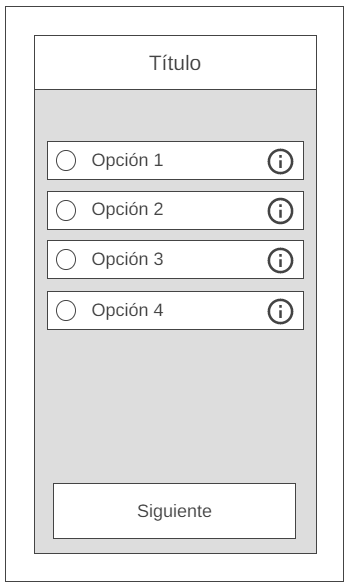
\includegraphics[scale=0.4]{Figures/Mockups/Mock_SeleccionUnica.png}
    \caption{Pantalla de selección única}
    \label{SeleccionUnica}    
\end{figure}

\subsubsection{Pantalla de selección única con grupos}
La vista de selección única con grupos es similar en funcionalidad a la pantalla de selección única, con una ligera diferencia.
Al acceder a la vista, los elementos que se muestran por pantalla son los diferentes grupos que forman parte de la etapa de creación
Al pulsar sobre uno de los grupos, éste se expande, mostrando todos los elementos contenidos en él (figura \ref*{SeleccionUnicaGrupos}). 
En caso de intentar abrir varios grupos, sólo quedará expandido el último seleccionado, quedando el resto contraídos, para facilitar la 
navegación por las distintas opciones de la etapa.

\begin{figure}[H]
    \centering
    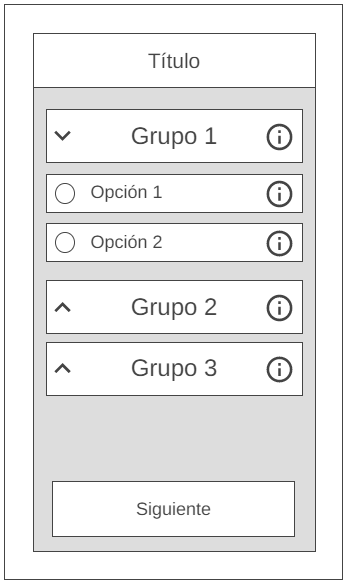
\includegraphics[scale=0.4]{Figures/Mockups/Mock_SeleccionUnicaGrupos.png}
    \caption{Pantalla de selección única con grupos}
    \label{SeleccionUnicaGrupos}    
\end{figure}
\newpage
\subsubsection{Pantalla de selección múltiple}
La vista de selección múltiple es una semejante a la vista de selección única, con la diferencia de que los círculos de selección 
se han sustituido por cajas de selección múltiple (figura \ref*{SeleccionMultiple}).

\begin{figure}[H]
    \centering
    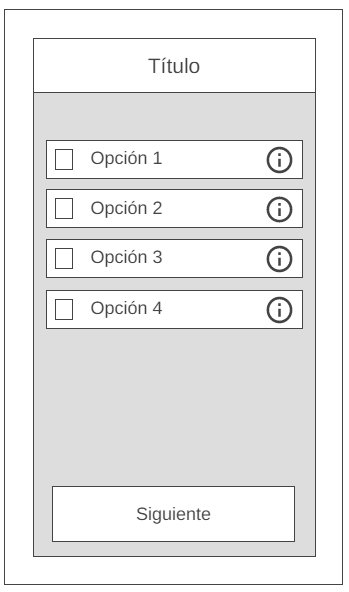
\includegraphics[scale=0.4]{Figures/Mockups/Mock_SeleccionMultiple.png}
    \caption{Pantalla de selección múltiple}
    \label{SeleccionMultiple}    
\end{figure}

\subsubsection{Pantalla de selección múltiple con grupos}
Esta vista es similar a la pantalla de selección única con grupos, habiendo sustituido los círculos de selección por 
cajas de selección múltiple (figura \ref*{SeleccionMultipleGrupos}).

\begin{figure}[H]
    \centering
    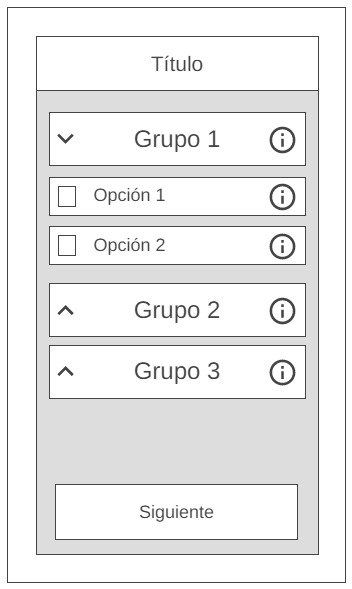
\includegraphics[scale=0.4]{Figures/Mockups/Mock_SeleccionMultipleGrupos.png}
    \caption{Pantalla de selección múltiple con grupos}
    \label{SeleccionMultipleGrupos}    
\end{figure}
\newpage
\subsubsection{Pantalla de gasto de puntos}
La vista de gasto de puntos muestra todos los elementos disponibles de una etapa de creación, y el valor del elemento 
que se desea añadir, acompañado por dos botones (de restar y sumar, respectivamente) para modificar dicho valor 
(figura \ref*{GastoPuntos}).

\begin{figure}[H]
    \centering
    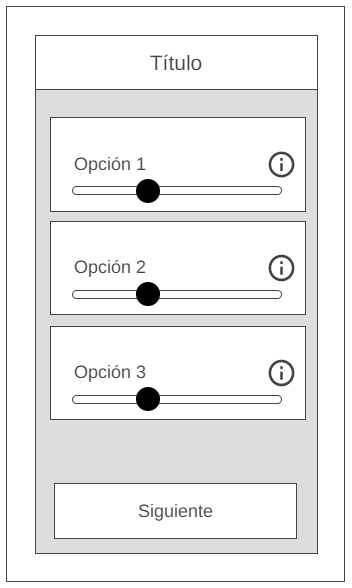
\includegraphics[scale=0.4]{Figures/Mockups/Mock_GastoPuntos.png}
    \caption{Pantalla de gasto de puntos}
    \label{GastoPuntos}    
\end{figure}

\subsubsection{Pantalla de gasto de puntos con grupos}
Esta vista funciona de la misma manera que la pantalla con gasto de puntos, pero incluyendo el trato de grupos del 
que disponen las pantallas de vista única y vista múltiple con grupos (figura \ref*{GastoPuntosGrupos}).

\begin{figure}[H]
    \centering
    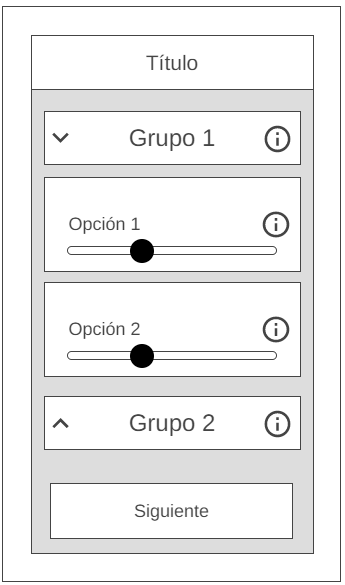
\includegraphics[scale=0.4]{Figures/Mockups/Mock_GastoPuntosGrupo.png}
    \caption{Pantalla de gasto de puntos con grupos}
    \label{GastoPuntosGrupos}    
\end{figure}
\newpage
\subsection{Pantalla de opciones del personaje}
Esta vista es muy sencilla, ya que solo muestra dos botones: uno para visualizar la información del personaje 
(\textit{Visualizar información}), y otro para calcular el valor de las habilidades del personaje (\textit{Calcular habilidad}), 
como se puede ver en la figura \ref*{OpcionesPersonaje}.

\begin{figure}[H]
    \centering
    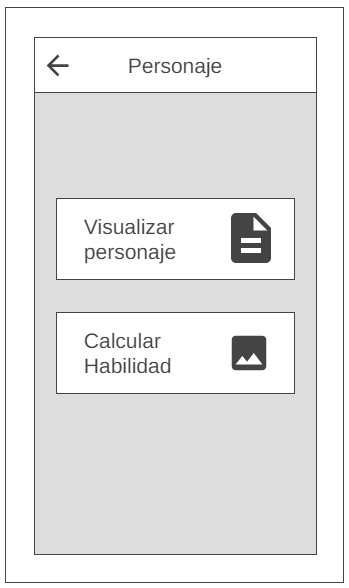
\includegraphics[scale=0.4]{Figures/Mockups/Mock_OpcionesPersonaje.png}
    \caption{Pantalla de opciones del personaje}
    \label{OpcionesPersonaje}    
\end{figure}

\subsection{Pantalla de campos del personaje}
En esta vista se muestran los diferentes campos de información de los que dispone el personaje.
Para visualizar uno de los campos, basta con seleccionarlo. La estructura es similar a la de la 
pantalla de inicio, a excepción de los iconos de la zona superior de la pantalla (figura \ref*{CamposPersonaje}).

\begin{figure}[H]
    \centering
    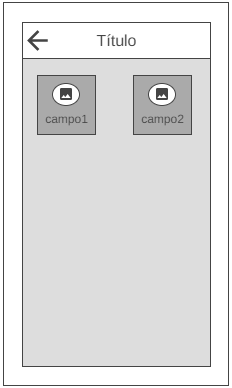
\includegraphics[scale=0.6]{Figures/Mockups/Mock_CamposPersonaje.png}
    \caption{Pantalla de campos del personaje}
    \label{CamposPersonaje}    
\end{figure}
\newpage
\subsection{Pantalla de información del personaje}
Esta vista muestra la información de uno de los campos del personaje, agrupada por secciones, tal y como 
se puede observar en la figura \ref*{InfoPersonaje}.


\begin{figure}[H]
    \centering
    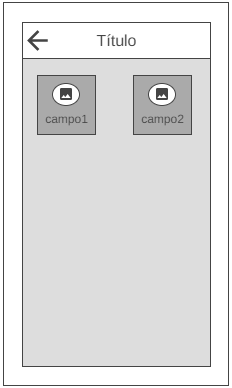
\includegraphics[scale=0.6]{Figures/Mockups/Mock_CamposPersonaje.png}
    \caption{Pantalla de información del personaje}
    \label{InfoPersonaje}    
\end{figure}

\subsection{Pantalla de cálculo de habilidad}
Finalmente, la vista de cálculo de habilidad permite seleccionar una habilidad del personaje y 
calcular el resultado total del intento del personaje al realizar dicha habilidad. La vista dispone de varios elementos, 
que se pueden apreciar claramente en la figura \ref*{CalculoHabilidad}.
\begin{itemize}
    \item Un botón de selección de habilidad.
    \item Un recuadro que indica la habilidad seleccionada.
    \item Un cuadro de texto para introducir el valor de una tirada de dados.
    \item Un botón para calcular el resultado de sumar el valor final de la habilidad del personaje al de la tirada.
\end{itemize}

\begin{figure}[H]
    \centering
    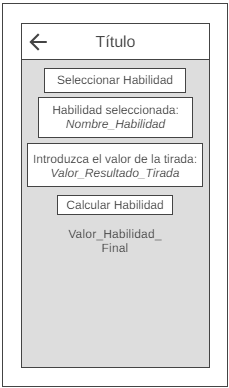
\includegraphics[scale=0.6]{Figures/Mockups/Mock_CalcularHabilidad.png}
    \caption{Pantalla de cálculo de habilidad}
    \label{CalculoHabilidad}    
\end{figure}
\newpage
\subsection{Pantalla de selección de habilidad}
La vista de selección de habilidad muestra las diferentes habilidades por las que el personaje podría 
realizar un cálculo de habilidad. Para seleccionar una, basta con pulsar el recuadro en el que se encuentra 
el nombre de dicha habilidad (figura \ref*{SeleccionHabilidad}).

\begin{figure}[H]
    \centering
    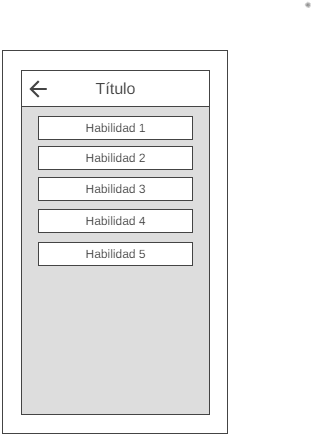
\includegraphics[scale=0.6]{Figures/Mockups/Mock_SeleccionHabilidad.png}
    \caption{Pantalla de selección de habilidad}
    \label{SeleccionHabilidad}    
\end{figure}

